\documentclass{article}
\usepackage{arydshln}
\usepackage[hidelinks]{hyperref}
\renewcommand{\baselinestretch}{1.5}
\usepackage[onehalfspacing]{setspace}
\setlength{\footnotesep}{0cm}
\usepackage[spanish]{babel}
\usepackage[utf8]{inputenc}
\usepackage{mathptmx}
\usepackage{courier}
\usepackage{helvet}
\usepackage[T1]{fontenc}
%\usepackage[paper=letterpaper,left=3cm,right=3cm,top=2cm,bottom=3cm]{geometry} 
\usepackage{framed,color}
\usepackage{graphicx}
\definecolor{shadecolor}{rgb}{0.1,0.1,0.1}
\usepackage{tocloft}
\renewcommand{\cftsecleader}{\cftdotfill{\cftdotsep}}
\usepackage{titlesec}
\titleformat{\section}{\normalfont\Large\bfseries\scshape}{\thesection.}{1em}{}
\titleformat{\subsection}{\normalfont\large\bfseries\scshape}{\thesubsection}{1em}{}
\usepackage[table]{xcolor}
\colorlet{tableheadcolor}{lightgray}
\usepackage{parskip}
\setlength{\parindent}{15pt}
\usepackage{multirow}
\usepackage{longtable}
\usepackage{pdfpages}
%\setcounter{tocdepth}{1}
\usepackage{float}
\restylefloat{table}
\usepackage{xstring}
\usepackage{titleps}

\newpagestyle{monstyle}{%
     \headrule
        \sethead{\thepage}
                   {}
                              {{\sectiontitle}}}

\begin{document}
\pagestyle{monstyle}
\title{Sistema de Información Geográfico Libre y Público para el Monitoreo Urbano\\
  (Objetivo Específico \#1)}
\author{Víctor Velásquez Solano}
\maketitle
\tableofcontents
\section{Introducción}

La importancia de conocer el contexto en el que se desarrollan los proyectos informáticos,
especialmente si son sociales (es decir, que la sociedad se ve afecta por el uso del producto), es
esencial para el desarrollo y subsistencia de los mismos. Si se desconoce la historia, los procesos,
la política y las necesidades sociales que han impulsado al desarrollo de determinadas herramientas,
entonces se transforman en proyectos carentes de motivo, si sólo se conocen las necesidades
inmediatas que está satisfaciendo la aplicación, entonces se prevé una corta vida del proyecto.
Además, tratar de conocer el contexto histórico, social y político al que pertenece la herramienta
de software genera una visión más completa que permitirá ofrecer un producto más acabado. Por lo
anterior, se reconoce al software como una herramienta que es incapaz de escapar al contexto en el
cual se desarrolla, razón por la cual es necesario clarificar tal contexto.

Este documento adscribe al Objetivo Específico 1 del proyecto de tesis que se titula ``Sistema de
Información Geográfico Libre y Público para el Monitoreo del Estado\footnote{Por necesidades del formato del título
del proyecto de tesis, la palabra ``estado'' comienza con mayúsculas, sin embargo, se refiere a la
``situación actual'', mas no a la institución social que forma parte de la estructura
político-social de las naciones actuales.} Urbano'', por tanto se requiere conocer los motivos que
obligan a los mecanismos gubernamentales actuales y otras instituciones a tener una visión del
estado del espacio urbano, qué realidad ha hecho que en Valdivia sea necesario recabar información
más allá de fuentes empíricas y el nexo que existe con la realidad de Chile y de América Latina,
puesto que, como se verá más adelante, la historia ha permeado de manera similar en los distintos
países latinoamericanos, sobre todo en materia urbanística. Se requiere además entender cuáles son
los conceptos relativos al urbanismo y los procesos de urbanización para luego entender la necesidad
que satisfacen y la funcionalidad de los Sistemas de Información Geográficos más allá de sus
aspectos técnicos.

El siguiente documento se divide en tres secciones, la primera es una introducción a los conceptos
de urbanismo y cuáles son las herramientas actuales que determinan y ayudan a identificar los
elementos espaciales que se consideran en el estudio urbano, especialmente enfocado en Chile. La
segunda sección del documento trata sobre el desarrollo del urbanismo en América Latina en general,
sin especificar en países en concreto, salvo algunas puntuales ocasiones donde se especifican datos
sobre Chile; la importancia de esta sección se debe a que ayuda a entender cuales son las
condiciones que motivan el surgimiento de este proyecto. La tercera sección de este documento cubre
aspectos más técnicos relacionados con los Sistemas de Información Geográficos, sus orígenes, su
utilización y sus componentes.

El propósito de este documento es de carácter introductorio, por tanto, la información que contempla
puede no estar acabada en su totalidad. Por lo anterior, este documento seguirá expandiéndose en el
desarrollo del Objetivo Específico 2 del proyecto de Tesis, el cuál centrará su desarrollo sobre el
contexto chileno.

\section{Urbanismo, urbanización y urbe}

\subsection{Definiciones generales}

Lo más lógico a la hora de recurrir a definiciones es la utilización del diccionario y a un proceso
de semiosis etimológica. A partir de esta semiosis es que se hace necesario identificar los
conceptos de urbe, urbanismos, urbanización, ciudad, barrio, por nombrar algunos.

Se tiende a diferenciar lo urbano de lo rural, considerando al primero relativo a la
urbe, es decir, ciudades altamente pobladas con una infraestructura servil a la interrelación de
determinados servicios sociales y las condiciones de esta infraestructura (porcentaje de calles
pavimentadas, acceso a hospitales, instituciones de educación entre otras características). Por
contra, se tiende a pensar en lo rural como lo campestre, bajos niveles de población, escaso acceso
a servicios de salud y educación, aislamiento de la ciudad. Sin embargo, la especificación sobre qué
es urbano y qué es rural es dinámica, es decir, varía acorde al tiempo y el territorio (legislación
país), pero siempre se consensúa que lo urbano es el complemento de lo rural en la distribución
espacial.

La urbanización es la ``Acción y efecto de urbanizar'', urbanizar es ``Hacer urbano, civilizar ||
Convertir un terreno en poblado abriendo calles y dotándolo de los servicios necesarios''. 
El urbanismo es el ``conjunto de conocimientos que se refieren al estudio de la creación,
desarrollo, reforma y progreso de los poblados en orden a las necesidades de la vida urbana''.

Al momento de concebir la función civilizadora de la urbanización se comprende que 
converge con otras disciplinas tales como la ingeniería civil, la arquitectura, la psicología, el
derecho, la lingüística, la antropología, la sociología, la semiótica y la política por nombrar algunas
\cite{Wkur}, puesto que el acto de civilizar es una tarea netamente cultural y que está sujeta a las
necesidades de la sociedad en determinado contexto. Está estrechamente relacionado con el desarrollo
y evolución del concepción de derechos de una determinada cultura, puesto que es el entendimiento y
satisfacción de estos derechos el que es determinante en la infraestructura urbana para asegurar el
bienestar de la población. Incluso, el concepto de urbanización y las métricas que determinan si un
espacio urbano cumple con las condiciones para considerarse como tal, más allá de la cantidad de
personas que conforman el poblado, van de la mano con el estudio de las condiciones
socio-económico-ambientales que tienen lugar dentro del mismo.


Acorde a lo anterior, se aprecia una marcada diferencia entre los conceptos de urbanismo y
urbanización, el urbanismo se dedica a la planificación del suelo interlocal, incluso abarcando
ámbitos de carácter rural, se dedica a la ordenación de las ciudades y del territorio.
La urbanización, por contra, se enfoca en los procesos constructivos, más
no con la ordenación urbana. Se podría hacer entendible esta diferencia abocando a que la
urbanización es la práctica del urbanismo.



\subsection{Definiciones de acuerdo a la legislación chilena}
\begin{quote}
\flushright{
\textit{
``Es evidente que la legislación urbana no puede seguir ignorando los derechos de las personas a tener
un lugar donde vivir con seguridad y dignidad. 
El impacto crítico de la desigualdad en la tenencia de la tierra en el entorno urbano exige que la
población urbana pobre tenga acceso a la información técnica necesaria para negociar mejor sus
inquietudes con los funcionarios públicos''
}
}

\textbf{Sonia Pereira}, Equidad en el acceso al suelo  para la población urbana pobre. 1997

\end{quote}

Las definiciones varían de un país a otro, sin ir más lejos y luego de las definiciones generales en
el capítulo anterior, se pueden identificar una serie de especificaciones frente a conceptos como la
urbanización, que también se entiende como el conjunto de viviendas situadas generalmente en un
antiguo medio rural junto a otras poblaciones\cite{Wkuv}.
En el plano nacional, de acuerdo a la Ordenanza General de Urbanismo y Construcciones, en el Capítulo 2: De las
Normas de Urbanización, artículo 2.2.1, se especifica lo siguiente:

\begin{quote}
``Se entiende por
urbanización la ejecución o ampliación de obras de infraestructura y ornato señaladas en el artículo
134 de la Ley General de Urbanismo y Construcciones, que se ejecutan en el espacio público
existente, al interior de un predio en las vías contempladas en un proyecto de loteo, o en el área
del predio que estuviere afectada a la utilidad pública por el Instrumento de planificación
Territorial respectivo.

La urbanización comprende dos tipos de gestión:
\begin{enumerate}
  \item La ejecución de obras de urbanización al interior de un predio por parte de su propietario.
  \item Le ejecución de obras de urbanización en el espacio público, por parte de los municipios u otros
        organismos públicos. ''
\end{enumerate}

En la misma Ordenanza General de Urbanismo y Construcciones, en el Título 1 ``Disposiciones
Generales'', Capítulo 1 ``Normas de competencia y definiciones'', Artículo 1.1.2; se pueden
encontrar las siguientes definiciones:

\begin{description}
  \item[Área rural:] territorio ubicado fuera del límite urbano.
  \item[Área urbana:] superficie del territorio ubicada al interior del límite urbano, destinada al
  desarrollo armónico de los centros poblados y sus actividades existentes y proyectadas por el
  instrumento de planificación territorial.
  \item[Área de extensión urbana:] superficie del territorio ubicada al interior del límite urbano,
  destinada al crecimiento urbano proyectada por el plan regulador intercomunal.
  \item[Barrio:] área habitacional, industrial, comercial o mixta que forma parte de una ciudad,
  compuesta generalmente de un grupo de manzanas con características similares.
  \item[Límite urbano:] línea imaginaria que delimita las áreas urbanas y de extensión urbana
  establecidas en los instrumentos de planificación territorial, diferenciándolos del resto del área
  comunal.
  \item[Límite de extensión urbana:] línea imaginaria que determina la superficie máxima destinada al
  crecimiento urbano proyectado por el plan regulador intercomunal.
  \item[Lote:] superficie de terreno continua resultante del proceso de división y urbanización del
  suelo, o de modificaciones, anexiones o sustracciones de la misma.
  \item[Sistema de Información Geográfica:] herramienta informática que permite el manejo de
  información planimétrica georeferenciada en interacción con bases de datos asociadas.
  \item[Urbanizar:] ejecutar, ampliar o modificar cualquiera de las obras señaladas en el artículo
  134 de la Ley General de Urbanismo y Construcciones que correspondan según el caso, en el espacio
  público o en el contemplado con tal destino en el respectivo instrumento de Planificación
  Territorial o en un proyecto de loteo.
\end{description}
\end{quote}

El Artículo 134 del párrafo 4$^{o}$ de la Ley General de Urbanismo y Construcciones dice lo
siguiente:

\begin{quote}
Para urbanizar un terreno, el           
propietario del mismo deberá ejecutar, a su costa, el      
pavimento de las calles y pasajes, las plantaciones y      
obras de ornato, las instalaciones sanitarias y            
energéticas, con sus obras de alimentación y desagües de 
aguas servidas y de aguas lluvias, y las obras de 
defensa y de servicio del terreno.

    Sin embargo, cuando las obras de alimentación y 
    desagüe que deban ejecutarse beneficien también a otros 
    propietarios, el servicio respectivo determinará el pago 
    proporcional que corresponda al propietario en estas 
    obras, en la forma que determine la Ordenanza General.
    
        Las plantaciones y obras de ornato deberán ser         
        aprobadas y recibidas por la Dirección de Obras            
        Municipales respectiva.                                    
\end{quote}

Mayores especificaciones sobre la legislación chilena relativa a materias de urbanismo, como el Plan
de Desarrollo Urbanístico Regional, plan Regulador y otros mecanismos provistos por el Ministerio de
Vivienda y Urbanismo o el Ministerio de Obras Públicas corresponden a una investigación posterior.

\subsubsection{Lo urbano y lo rural acorde al Censo chileno}

El censo es el padrón de la población nacional, para que sea llevado a cabo se define una división
geográfica censal que debe ser operativa, homogenea, representativa y de codificación única. Esta
estructura queda representada en la figura~\ref{censo}, que nos entrega una rápida descripción de la
división territorial chilena. 

\begin{figure}
  \centering
  \caption{División territorial censal}
  \label{censo}
  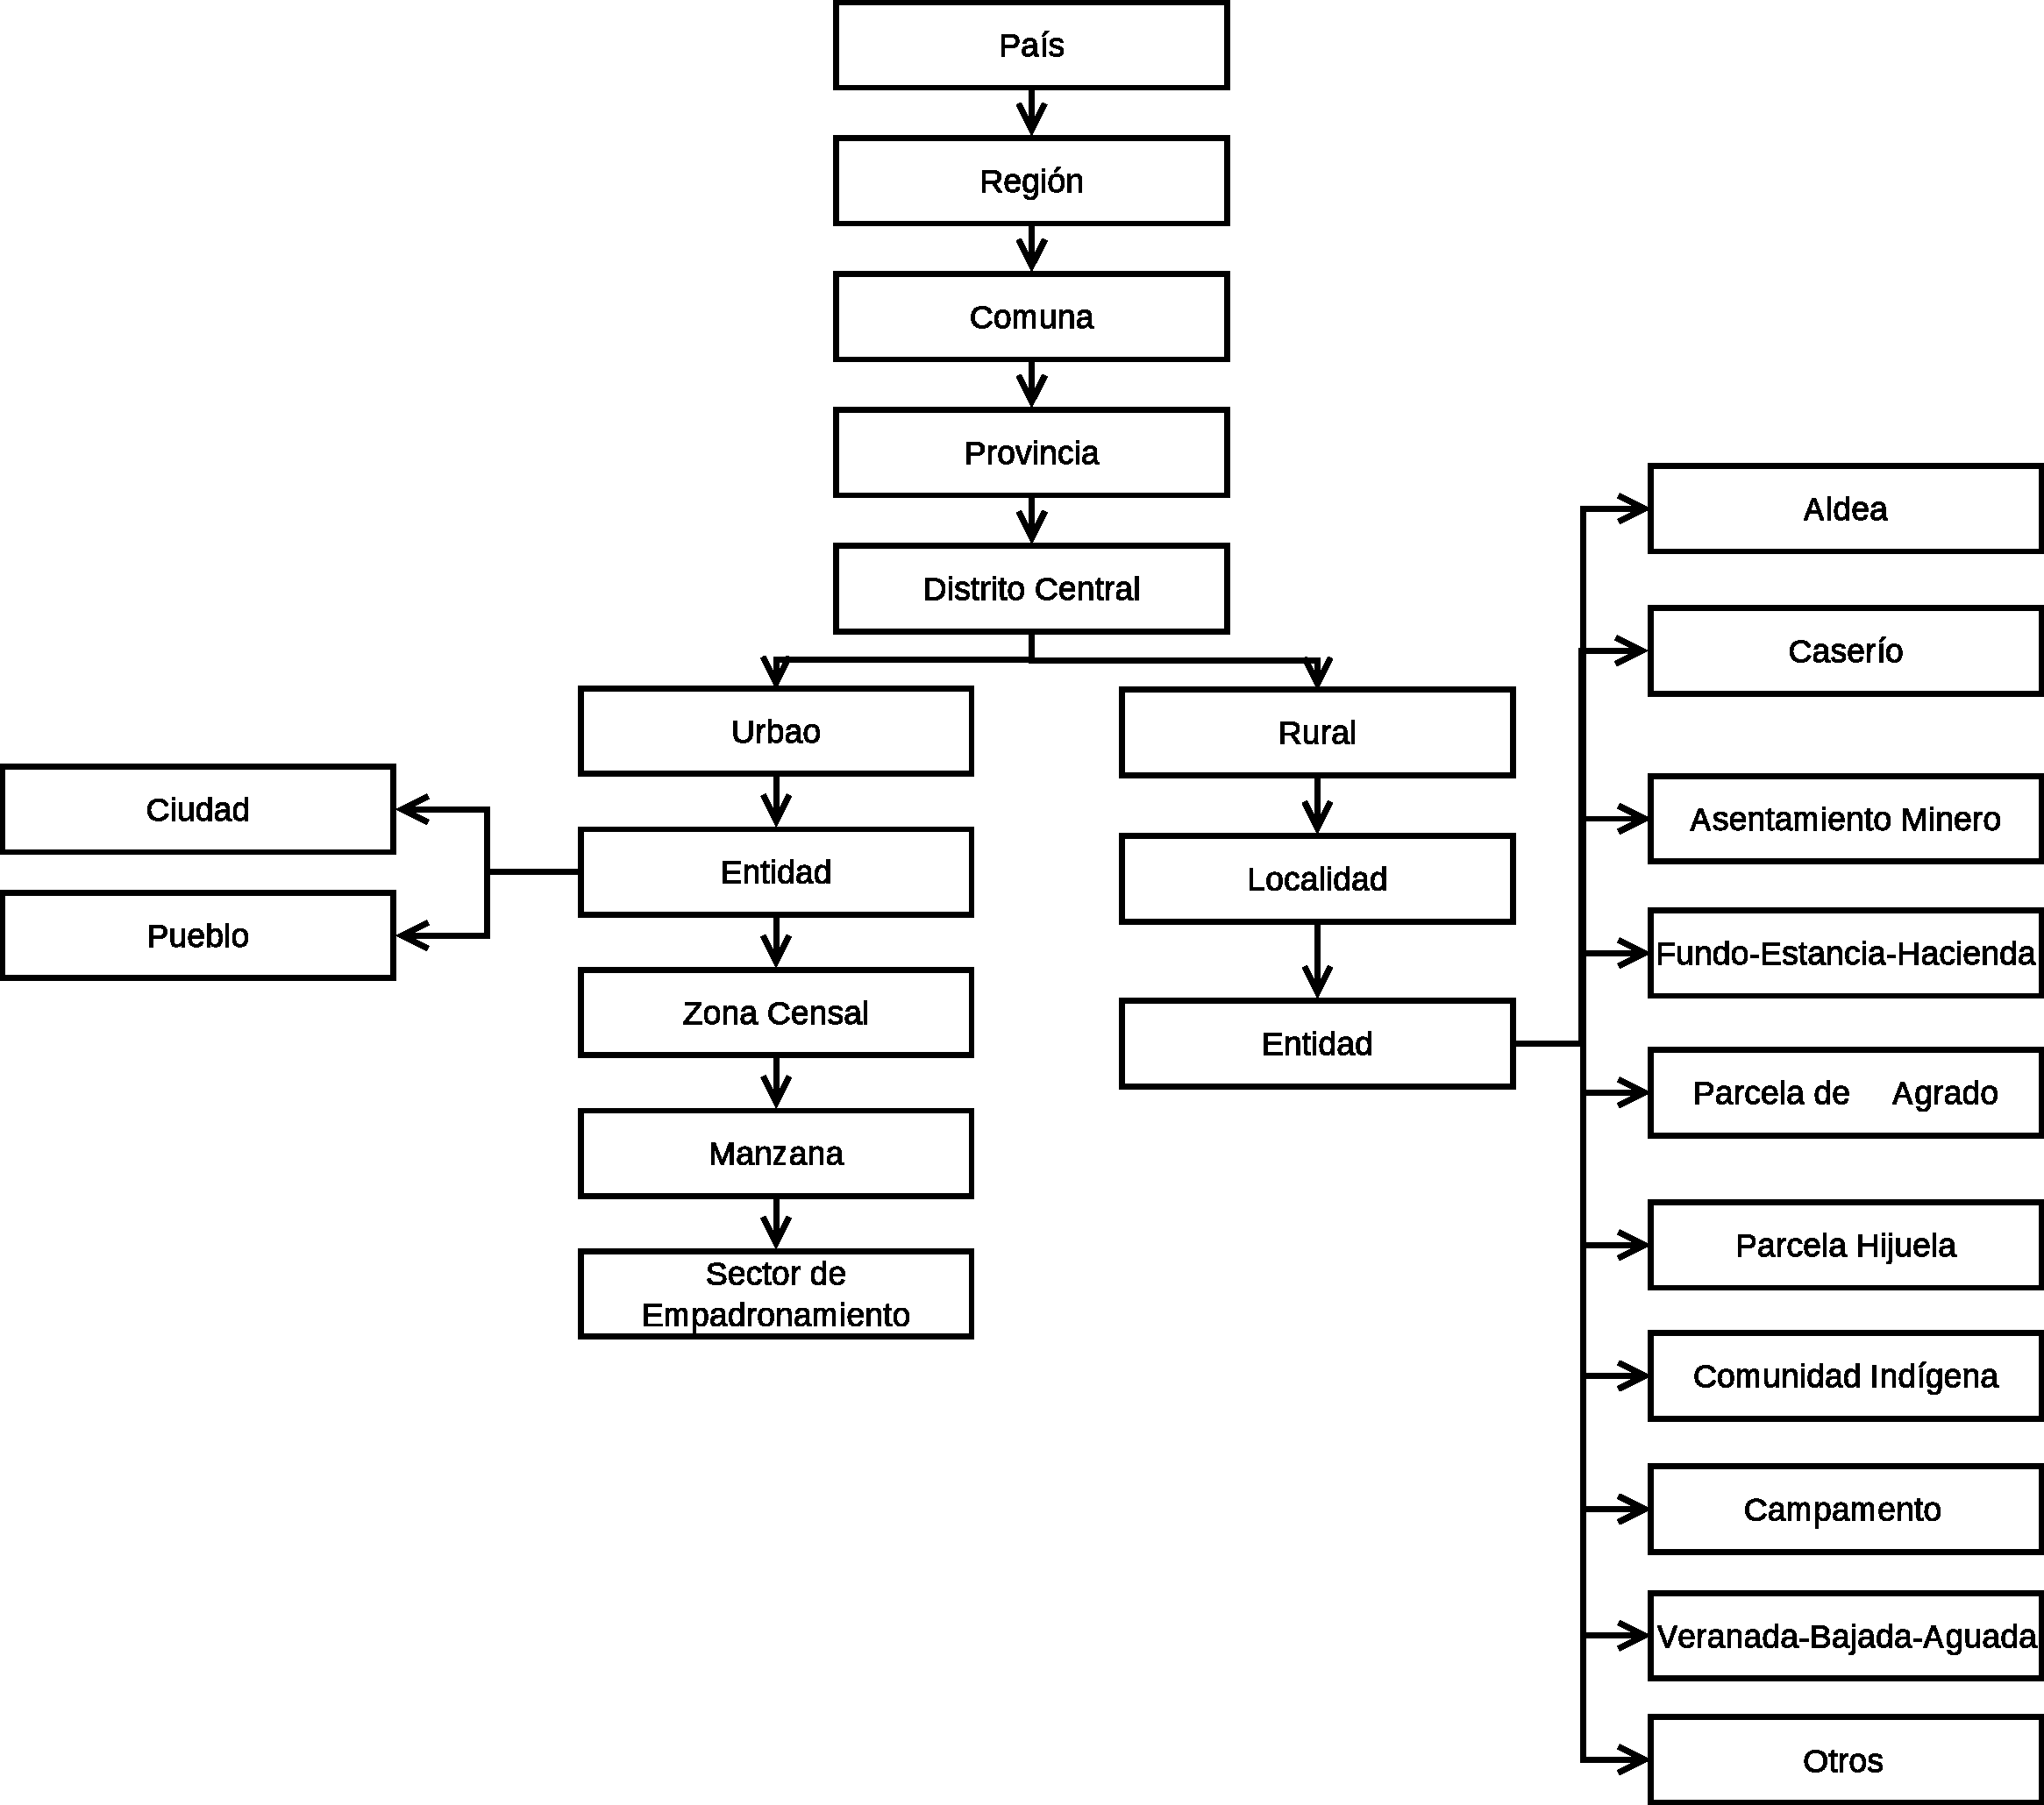
\includegraphics[scale=0.25]{censo}
\end{figure}

El INE ha definido la conformación del distrito censal, que es la unidad
geográfica que subdivide a la comuna con fines censales en dos áreas: (1) área urbana y (2) área
rural, estas áreas son dicotómicas, es decir, lo urbano es lo contrario a lo rural. Sin embargo,
como ya se ha mencionado con anterioridad en este documento, los conceptos de urbano y rural varían
de acuerdo al tiempo. De este modo es como podemos distinguir las siguientes definiciones que ha
hecho el INE para los distintos censos desde 1960 hasta el 2002 relativas a lo urbano:

\begin{description}
  \item[Censo 1960:] Todas las poblaciones del país con características urbanas (ciudades, pueblos,
  aldeas, minerales, salitreras y otros centros poblados con dichas características, como bases
  aereas, campamentos, etc) ya sean concentradas con algunas calles pavimentadas o con algunos
  servicios de utilidad pública.
  \item[Censo 1970:] Área que presenta un límite mínimo de 40 viviendas continuas o agrupadas, con
  definición preestablecida de calles y que además cuenta con alguno de los siguientes servicios:
  carabineros, correo, luz eléctrica, agua potable, alcantarillado, comercio establecido, escuela.
  \item[Censo 1982:] Todo lugar habitado que presenta rasgos de urbanización, al menos incipiente,
  idependientemente de la actividad que desarrollan sus habitantes, y que cuenta con un mínimo de 60
  viviendas agrupadas y contiguas, siempre que su población no sea inferior a 301 habitantes.
  Excepciones: aeropuertos, centros de turismo y esparcimiento y caseríos cordilleranos altiplánicos
  del Norte Grande que no alcancen los montos mínimos de población y vivienda establecidos.
  \item[Censo 1992:] Conjunto de viviendas concentradas con más de 2.000 habitantes , o entre los
  1.001 y 2.000 habitantes, con el 50\% o más de su población económicamente activa dedicadas a las
  actividades secundarias y/o terciarias. Excepcionalmente, los centros que cumplen funciones de
  turismo y recreación con más de 250 viviendas concentradas y que no alcanzan el requisito de
  población que se consideran urbanos.
  \item[Censo 2002:] Conjunto de viviendas concentradas con más de 2.000 habitantes, o entre 1.001 y
  2.000 habitanes, con el 50\% o más de su población económicamente activa dedicadas a las
  actividades secundarias y/o terciarias. Excepcionalmente los centros que cumplen funciones de
  turismo y recreación con más de 250 viviendas concentradas y que no alcancen el requisito de
  población se consideran urbanos.
\end{description}

\section{La urbanización en América Latina}

Para efectos de este apartado del documento se restringirá la urbanización a sus dimensiones
demográficas, es decir, el aumento de la población en las áreas urbanas o el aumento del nivel o
grado de urbanización (expansión de las ciudades). Además, vale destacar que si bien se encontrarán
puntos comunes en cuanto al desarrollo de la urbanización en América Latina, cada país tiene sus
propias definiciones nacionales que afecta en como éstas crecen y como son consideradas.

\subsection{Contexto Mundial}
``En la actualidad América Latina muestra un nivel de urbanización de un $73.5\%$, cercano al conjunto
de las regiones más desarrolladas\cite{Lattes}.''

\begin{table}
  \centering
  \caption{Nivel de Urbanización de las grandes regiones del mundo desde 1925 y proyección al 2025
  (Porcentajes)
  }
  \label{latammundo}
  \begin{tabular}{|llllll|}
    \hline
    \textbf{Regiones} & 1925 & 1950 & 1975 & 2000 & 2025 \\
    \hline
    Total Mundial &  20,5 &29,7 &37,9 &47,0 &58,0 \\
    \hline
    Regiones más desarrolladas &  40,1 &  54,9 &  70,0 &76,0 &82,3 \\
    Regiones menos desarrolladas &  9,3 &17,8 &26,8 &39,9 &53,5 \\
    \hline
    África &  8,0 &14,7 &25,2 &37,9 &51,8 \\
    América Latina &  25,0 &41,4 &61,2 &75,3 &82,2 \\
    América del norte &  53,8 &63,9 &73,8 &77,2 &83,3 \\
    Asia &  9,5 &17,4 &24,7 &36,7 &50,6 \\
    Europa &  37,9 &52,4 &67,3 &74,8 &81,3 \\
    Oceanía &  48,5 &61,6 &71,8 &70,2 &73,3 \\
    \hline
  \end{tabular}
\end{table}

Como se puede ver en el cuadro~\ref{latammundo} la urbanización en América Latina ha ido creciendo aceleradamente. Aunque, como se
verá más adelante, este crecimiento no significa que las condiciones de vida de los habitantes vayan
mejorando, en un informe de CEPAL del año 2000 se indica la tendencia al alza de personas pobres. La
pobreza en América Latina forma parte de un problema urbano, de un 37\% de residentes urbanos pobres
para 1970, se eleva a la cifra de el 62\% para el año 1999.

Observando los niveles y tendencias de urbanización de los veintidós países con mayor población de
América Latina que aparecen en el cuadro~\ref{porpais} se percibe la diversidad de las
situaciones  que envuelven a cada país. En el año 1950, sólo en tres países más del 50\% de la
población residía en áreas urbanas (Chile, Uruguay y Argentina), en cambio, para el año 2010, solo
dos países (Haítí y Guatemala) todavía no superan ese 50\%. Por lo demás, las tasas de crecimiento
de los niveles de urbanización son irregulares entre todos los países.

\begin{table}
  \centering
  \caption{Nivel de Urbanización por país en América Latina}
  \label{porpais}
  \begin{tabular}{|llllllllll|}
  \hline
  País & & & & & & & & & \\
  & 1950& 1960& 1970& 1980& 1990& 2000& 2010& 2020& 2030 \\
  \hline
  Uruguay &78,0 &80,1 &82,1 &85,2 &88,7 &91,2 &93,0 &94,1 &94,7\\ 
  Argentina &65,3 &73,6 &78,4 &82,9 &86,5 &89,9 &92,0 &93,1 &93,9\\ 
  Venezuela &46,8 &61,2 &71,6 &79,4 &84,0 &86,9 &89,1 &90,7 &91,8\\ 
  Chile &58,4 &67,8 &75,2 &81,2 &83,3 &85,7 &87,8 &89,5 &90,7\\ 
  Brasil &36,0 &44,9 &55,8 &66,2 &74,7 &81,3& 85,2 &87,3 &88,9\\ 
  Cuba &49,4 &54,9 &60,2 &68,1 &73,6 &75,3 &77,3 &79,7 &82,3\\ 
  Puerto Rico &40,6 &44,5 &58,3 &66,9 &71,3 &75,2 &78,5 &81,3 &83,6\\ 
  México &42,7 &50,8 &59,0 &66,3 &72,5 &74,4 &76,7 &79,3 &81,9\\ 
  Colombia &37,1 &48,2 &57,2 &63,9 &69,5 &73,9 &77,6 &80,5 &83,0\\ 
  Perú &35,5 &46,3 &57,4 &64,6 &68,9 &72,8 &76,3 &79,3 &81,9\\ 
  Ecuador &28,3 &34,4 &39,5 &47,0 &55,1 &65,3 &73,1 &77,8 &80,6\\ 
  R. Dominicana &23,8 &30,2 &40,3 &50,5 &58,3 &65,1 &70,5 &74,5 &77,7\\ 
  Bolivia &37,8 &39,3 &40,7 &45,5 &55,6 &62,5 &67,8 &72,1 &75,7\\ 
  Panamá &35,8 &41,3 &47,7 &50,5 &53,7 &56,2 &59,6 &64,0 &68,6\\ 
  Nicaragua &34,9 &39,6 &47,0 &50,3 &53,1 &56,1 &60,3 &65,1 &69,5\\ 
  Jamaica &26,7 &33,8 &41,5 &46,8 &51,5 &56,1 &61,0 &65,9 &70,3\\ 
  Paraguay &34,5 &35,6 &37,1 &41,7 &48,7 &56,0 &62,3 &67,3 &71,5\\ 
  Honduras &17,6 &22,8 &28,9 &34,9 &41,8 &52,7 &61,2 &66,7 &71,0\\ 
  Costa Rica &33,5 &36,6 &39,7 &43,1 &45,8 &47,8 &51,2 &56,0 &61,4\\ 
  El Salvador &36,5 &38,4 &39,4 &41,6 &43,9 &46,6 &51,0 &56,6 &62,0\\ 
  Guatemala &29,5 &32,5 &35,5 &37,4 &38,1 &39,7 &43,5 &49,4 &55,4\\ 
  Haití &12,2 &15,6 &19,8 &23,7 &29,5 &35,7 &42,3 &48,8 &54,9\\ 
  Total &41,4 &49,3 &57,5 &65,0 &71,1 &75,4 &78,6 &81,1 &83,3 \\
  \hline
  \end{tabular}
\end{table}

Si se agrupan los 22 países en seis subregiones geográficas y se ordenan a
éstas por su nivel de urbanización actual (Cuadro~\ref{regioneslatam}) se puede ver que América
Central es la única subregión que aún muestra predominio de población rural
(nivel de urbanización del 47,8 por ciento). El Caribe (61,8 por ciento),
con un nivel medio de urbanización, se caracteriza, además, por una gran diferencia
interna: Cuba (75,3 por ciento) en un extremo y Haití (35,7) en el
otro. México y la subregión Andina con promedios altos, incluyendo esta subregión 
países con marcadas diferencias de nivel: por un lado Ecuador (65,3
por ciento) y por el otro Venezuela (86,9 por ciento). Brasil, el país de mayor
tamaño, también alcanza niveles altos de urbanización y, por último, el Cono
Sur relativamente homogéneo en tres países (Uruguay, Argentina y Chile) y
con un país muy desigual (Paraguay), aparece como la subregión más urbanizada
de América Latina (85,9 por ciento) en el presente.

\begin{table}
  \centering
  \caption{Niveles de urbanización por subregiones geográficas, América Latina año 2000}
  \label{regioneslatam}
  \begin{tabular}{|lc|}
    \hline
    Subregiones/Países & Nivel de urbanización año 2000 (porcentajes)\\
    \hline
    América Central &47,8\\
    \hline
    Nicaragua &56,1\\
    Panamá &56,2\\
    Costa Rica &47,8\\
    El Salvador &46,6\\
    Honduras &52,7\\
    Guatemala &39,7\\
    \hline
    Caribe &61,8\\
    \hline
    Cuba &75,3\\
    Puerto Rico &75,2\\
    R. Dominicana &65,1\\
    Jamaica &56,1\\
    Haití &35,7\\
    \hline
    México &74,4\\
    \hline
    Subregión Andina &74,6\\
    \hline
    Venezuela &86,9\\
    Colombia &73,9\\
    Perú &72,8\\
    Bolivia &62,5\\
    Ecuador &65,3\\
    \hline
    Brasil &81,3\\
    \hline
    Cono Sur &85,9\\
    \hline
    Uruguay &91,2\\
    Argentina &89,9\\
    Chile &85,7\\
    Paraguay &56,0\\
    \hline
  \end{tabular}
\end{table}

Estos son, a grandes razgos, los niveles de urbanización en América Latina.

\subsection{Contextos Regional (América Latina)}

A continuación se expone una serie de citas a artículos relativos al desarrollo del urbanismo en
América Latina pertenecientes a la ``Serie Población y Desarrollo: Urbanización, redistribución
espacial de la población y transforamciones socioeconómicas en América Latina (José Marcos Pinto da
Cunha)'' y el compilado de artículos ``Perspectivas urbanas, temas críticos en políticas de suelo en
América Latina'' de varios autores  pertenecientes al Instituto Lincoln de Políticas de Suelo.

El orden de esas citas es intencional, para dar una congruencia con el texto. Estos extractos fueron
seleccionados dado que presentan una imagen del desarrollo urbanístico en la región y se relacionan
con el proyecto de software.


\subsubsection*{CEPAL: I. Urbanización en América Latina en tiempos de globalización: elementos para el debate}
  Es interesante señalar que no existe un consenso con respecto a la globalización, tanto en lo que se
  refiere al concepto como a sus implicaciones; y así lo muestra Wong-Gonzales\cite{Won99} cuando señala que lo
  más interesante es su carácter ``altamente contradictorio y paradójico'' que se refleja también en
  las tendencias espaciales derivadas de esta nueva etapa del capitalismo.

  Sin embargo, la literatura registra varios elementos recurrentes sobre las caracterísitcas de este
  proceso llamado ``capitalismo tardío''. Las más interesantes para este análisis parecen ser:
  \begin{itemize}
    \item Modificación de ciertas especialidades vigentes en el período fordista;
    \item Reestructuración productiva: emergencia de un sistema de producción flexible y menos
    dependiente de localizaciones espaciales específicas;
    \item Reorganización de las estructuras espaciales y creación de nuevos espacios para la
    producción, lo que da origen al debate sobre concentración/desconcentración;
    \item Revalorización del espacio local/regional;
    \item Disminución de control del Estado sobre el espacio y el tiempo;
    \item Transformación significativa en la división regional y en el perfil del mercado de trabajo.
  \end{itemize}

  [\ldots]

  El carácter contradictorio de la globalización en cuanto al territorio queda claro en esta cita:
  ``No obstante esta tendencia de deterritorialización propia de los procesos de globalización y
  virtualización, se presenta simultáneamente una tendencia a la reterritorialización. Este es un
  reflejo más del carácter altamente paradójico de los fenómenos señalados. La primera tendencia alude
  a la emergencia de sistemas globales que escapan a las determinaciones específicas de territorios
  particulares; la segunda se refiere al carácter de producción definen los roles de espacios locales;
  al mismo tiempo, características específicas de territorios particulares se vuelven requisitos
  fundamentales para la competitividad global" (Wong-Gonzáles \cite{Won99}).

  [\ldots]

  Según De Mattos, en Chile la desconcentración se registró en el periodo anterior a la
  reestructuración económica postindustrialización sustitutiva con la ``aplicación de un importante
  paquete de políticas de liberalización y desregulación''. De la misma manera que en el citado
  análisis, otros autores sostienen que la globalización favorece a los grandes centros urbanos:

  \textit{``Globalization reinforces the advantages of large urban areas. Globalization implies
  international specialization and trade resulting from electronic communication and reduced
  governmment barriers. Thes processes will spread the benefits of large urban areas to developing
countries''\cite{Mil00}.}

  Tales ventajas no implican necesariamente una mayor concentración, especialmente de las actividades
  productivas del sector industrial. Como explica Wong-Gonzales \cite{Won99} ``las tendencias de dispersión
  o de concentración, no pueden ser generalizadas'' toda vez que ``ellas varían de un sector
  productivo a otro y aún entre los distintos segmentos productivos de un mismo sector \ldots''
  Además, el autor enfatiza que los patrones de dispersión/concentración tabién pueden variar en
  el tiempo, lo que muestra la dificultad de establecer un patrón único para los impactos
  territoriales de la globalización.

  Con estos ejemplos queda claro que, siendo verdad que la globalización puede tener efectos distintos
  dependiendo de las características del país y de su aparato productivo, lo valedero son sus impactos
  decisivos sobre los principales centros urbanos en términos de su estructura productiva y, por ende,
  en el mercado de trabajo, con implicaciones en la propia dinámica demográfica y migratoria.
  Castelles\cite[Cas99] afirma ``en cualquier proceso de transición histórica, una de las expresiones de
  cambio sistémico más directo es la transformación de la estructura ocupacional, es decir, de la
  composición de las categorías profesionales y del empleo''. Varios de los
  estudios centrados en el mercado del trabajo y sus transformaciones en la era de la globalización
  coinciden en destacar el cambio radical de ese mercado en Latinoamérica. Como señala Gwynne
  \cite{Gwy99},
  las reformas neoliberales -y la consecuente apertura comercial- adoptada por los países para
  enfrentar sus crisis fiscales a comienzos del decenio de 1980 tuvieron impactos importantes sobre el
  mercado de trabajo, en particular en materia de empleo formal (muy bajo dinamismo) y desempleo
  (aumento significativos).

  [\ldots]

  Al comparar entre los países desarrollados y los latinoamericanos podía pensarse que las
  transformaciones económicas -y los desajustes que ellas provocan en el empleo- demandarían sólo
  algún tiempo para que los trabajadores se ajustasen a las nuevas demandas del mercado. Pero hasta el
  momento la situación es bien diferente, pues aumento la expulsión de los trabajadores del sector
  formal hacia una situación de informalidad, con un pasaje eventual por el desempleo abierto, a lo
  que se denomina a veces ``informalización'' y otras ``precarización'' \cite{Ded99}.

  [\ldots]

  Es indiscutible que la globalización provoca impactos en la creación de nuevas espacialidades, o
  ``espacios de la globalización'' \cite{Bae99}. Sin embargo, existen dudas sobre sus impactos -o
  mejor dicho, su magnitud- sobre el tejido intraurbano. Beaninger (1999) revive la contribución de
  Gottdiener al debate cuando señala que este autor reconoce el impacto de las transformaciones
  contemporáneas en el espacio urbano y sostiene que las nuevas formas espaciales observadas en los
  Estados Unidos -que es su estudio de caso- fueron provocadas por factores presentes desde mucho
  tiempo en la sociedad. Sin embargo, este autor, según Baeninger, reconoce que esa nueva etapa del
  capitalismo tuvo implicaciones decisivas en el tejido social de los centros urbanos. Al igual que
  Castelles \cite{Cas89} reconoce que la reestructuración productiva promovió y continúa forzando mediante,
  por ejemplo, la precarización del trabajo, la dualización de la sociedad. Y quizás ésta sea una de
  las principales implicaciones del proceso en cuanto a entender fenómenos actuales como la
  metropolización, la periferización y otros.

  Cuando más se piensa en la dinámica demográfica intraurbana o intrametropolitana -o, de manera más
  general, en la expansión urbana de América Latina- surgen dos cuestiones: i) el patrón ``periférico
  del crecimiento -caracterizado por la ubicación de la población con bajos recursos en áreas cada vez
  más lejanas de los centros valorizados- y, como consecuencia, ii) el sostenido proceso de
  segregación espacial.

  Villa y Rodriguez \cite{Rod97} señalan que ``uno de los temas que provoca mayor inquietud entre los
  planificadores, urbanos\ldots es la expansión física de las metrópolis de América Latina \ldots El
  aumento de la superficie es un proceso complejo impulsado por diversos factores, entre los que
  destacan: i) las modalidades informales de ocupación de suelos por los asentamientos populares, ii)
  el uso especulativo del suelo por empresas inmobiliarias y iii) la acción pública destinada a
  proveer vivienda a los sectores de menor ingreso''.

  Lo cierto es que el proceso de metropolización representó en los países latinoamericanos una
  agudización de la diferenciación socioespacial en el contexto intraurbano, ya que las periferias
  ``son la materialización de mecanismos de exclusión/segregación'', que pueden expresarse en las
  malas condiciones de habitación, transportes, infraestructura urbana, etc. \cite{Pav96}.

  [\ldots]

  Otra tendencia es la agudización de la fragmentación del espacio, a través de su apropiación para
  trabajar, entretenerse, vivir, consumir. Concordando con la visión de que el
  fenómeno de la expansión urbana no es en nada novedoso, De Mattos señala que la aplicación de
  políticas de liberalización económica y de desregulación logró ``despejar el camino para la
  afirmación de una lógica estrictamente capitalista en la producción y reproducción metropolitana''.

  Ambos autores, y a ellos se suma Gottdienes, coinciden en que la transformación del espacio en una
  mercancía, la supremacía de su valor de uso sobre su valor de cambio 
  o, dicho de otra forma, la pérdida de importancia de su función social, llevaron a la
  desorganización o el desorden en el tejido urbano, lo que segregó cada vez más a la población. En
  ese sentido, el papel del poder público, y particularmente su omisión, a veces por negligencia y a
  veces por falta de condiciones financieras, especialmente después de la crisis fiscal del decenio
  1980 contribuyó mucho a esta situación.

  [\ldots]
  
  Al contrario de lo que sucedió hace algunas décadas, las tendencias urbanas -y particularmente las
  metropolitanas más actuales- muestran una redefinición del significado de la periferia y, por que
  no, del espacio rural. Aparecen asentamientos urbanos distantes de los centros dedicados a la
  población de más alta renta (condominios cerrados, ``country-clubs'', etc.), que resultan de
  motivaciones opuestas a las que condicionan la periferización de la población pobre, es decir, mejor
  calidad de vida, mayor seguridad, mayor contacto con la naturaleza, etc.

  En la metrópolis contemporánea latinoamericana, la periferización dejó de ser un fenómeno asociado
  únicamente a los desplazamientos de la población de baja renta hacia espacios alejados y menos
  valoralizados. En su acepción más utilizada ocurre en los centros de varias áreas metropolitanas,
  -viviendas ``subnormales'' (``villas miseria'', ``favelas'', ``conventillos'') y ocupaciones
  irregulares- y en la medida en que la oferta de habitación disminuyó mucho en función no sólo de la
  perdida de poder de financiamiento del Estado sino también del empobrecimiento sostenido de la
  población.

\subsubsection*{CEPAL: II.\@ Aspectos Metodológicos de la investigación}
  Antes de entrar al análisis empírico de las tendencias y especificaciones de la urbanización en
  América Latina es importante dejar en claro algunas dificultades metodológicas que surgen de las
  particularidades de la información utilizada: La información se obtiene en base a recuperación de
  censos, con las diferencias de los canales censales entre los varios países; la inexistencia de
  series históricas completas para algunos de ellos, y los consiguientes desajustes temporales;
  diferencias de definiciones (como las de zonas urbanas y rurales); 

  \subsubsection*{Informalidad, regularización y Derecho de propiedad (Isabel Viana)}  
  América Latina es una de las zonas más urbanizadas del planeta: tres de cada cuatro latinoamericanos
  viven en ciudades, y se estima que casi un 44\% de la población urbana de la región vive en áreas
  informales. Pero la pobreza urbana no se concentra solo en los sectores de alta precariedad, ni
  tampoco son l¿pobres todos los hogares que viven en los tugurios. La informalidad creciente, aún en
  circunstancias de recuperación económica, es tema central de la agenda latinoamericana por sus
  implicancias en la calidad de vida de los que viven en áreas de urbanización precaria, las
  disfunciones que genera en toda la sociedad urbana, los compromisos ambientales que conlleva y los
  problemas de gestión urbana que genera. La compresión ajustada del fenómeno es la única vía válida
  para definir intervenciones apropiadas.

  [\ldots]

  Martin Somlka y Cláudia Damasio definen el alcance, la profundidad y las consecuencias
  nocivas del proceso de crecimiento de la ciudad informal en América Latina. Ellos definen la
  informalidad como fenómeno multidimensional que involucra problemas relacionados con la propiedad
  del suelo urbano, las normas y regulaciones vigentes, el número y calidad de los servicios
  provistos, la calidad ambiental del área en que tiene lugar el asentamiento y el proceso de
  ocupación en si mismo. Este se opone al proceso formal de desarrollo urbano, en el que la ocupación
  es la culminación de la secuencia legal y regulada de obtención de capacidades para planificar,
  demarcar, construir infraestructuras y todas de servicios a cierta pieza urbana.

\subsubsection*{Uso de suelo y desarrollo urbano (Eduardo Reese,  colaborador Juan Ignacio Duarte)}
Efectivamente, a partir de los años noventa la lógica interna de producción y reproducción de las
ciudades latinoamericanas experimenta cambios significativos, y el tipo predominante de gestión de
la mayoría de los consumos colectivos urbanos estrecha sus vínculos con el mercado. La expresión más
cabal de este proceso es la privatización de cada vez más amplios sectores de nuestras ciudades con
un masivo efecto diferenciadior sobre la estructuración del territorio urbano. De tal forma, se
verifica una acentuación de la fragmentación del espacio urbano en coincidencia con los procesos de
agudización de las desigualdades socioeconómicas y un cambio del patrón tradicional de segregación
socioespacial.

Esta nueva situación reaviva con fuerza y justifica el renovado interés por el manejo del suelo como
pieza estratégica dentro del abanico de las políticas públicas territoriales. 

En esa línea de pensamiento, en todos los trabajos aparece subyacente otra coincidencia, como es la
necesidad de mejorar los instrumentos de gestión y de regulación a fin de fortalecer la acción
pública de los gobiernos municipales para corregir los efectos negativos producidos por el
funcionamiento de los mercados de suelo. En esta coincidencia de base, los autores bien podrían
estar sintetizados por las palabras de Jordi Borja: ``Los efectos perversos del mercado sobre la
ciudad no son fatales sino resultado de opciones políticas perversas''.

[\ldots]

Un caso particular en el contexto de las experiencias latinoamericanas lo constituye la experiencia
chilena de la liberalización del mercado de suelo. Como plantean Martim Smolka y Francisco Sabatini,
las medidas de corte neoliberal tomadas en relación con el mercado de tierras generaron una
expansión descontrolada de la urbanización a la vez que estimularon el alza de los precios y la
segregación de los sectores más pobres. Incluso en la actualidad, el incremento de los precios del
suelo está absorbiendo una proporción cada vez mayor del subsidio a la vivienda otorgado por el
gobierno chileno.

\subsubsection*{Expansión urbana y regulación del uso del suelo en América Latina (Mario Lungo)}
Una serie de cambios demográficos y económicos están marcando la expansión de varias clases de
nuevos conjuntos residenciales en América Latina. Desde grandes proyectos para sectores sociales de
ingresos medios y bajos hasta las exclusivas ``urbanizaciones enrejadas'' para los grupos de altos
ingresos, a veces estas áreas residenciales coexisten con grandes centros comerciales situados a lo
largo de las autopistas principales. No obstante, en los asentamientos pobres de las ciudades
latinoamericanas persiste la falta de equipamientos y servicios urbanos como transporte público,
suministro de agua municipal, alcantarillado y vías de acceso adecuadas.

La tendencia hacia la expansión en esas áreas periféricas sobrevaluadas pero al mismo tiempo
carentes de servicios contrasta con la reducción de la actividad residencial en áreas centrales
provistas de equipamientos y servicios básicos. Conforme estas zonas urbanas de suelo subutilizado y
vacante se vuelven menos pobladas y más devaluadas, el ciclo de deterioro va empeorando. La
enigmática relación que hay entre el control de la expansión territorial y el apoyo de la
densificación urbana es un punto clave del debate sobre regulación del usuo del suelo entre
especialistas formuladores de políticas latinoamericanos, y lleva tres asuntos de política de suelo
relacionados: el deterioro del medio ambiente, la conservación de centros históricos de las ciudades
y la competitividad de las ciudades.

\subsubsection*{El debate sobre la liberalización del mercado en Chile}

Pocos países de América Latina o del resto del mundo se han atrevido a poner en práctica reformas
tan radicales de la política de tierras urbanas como lo ha hecho Chile en los últimos 20 años. En
1979 el gobierno comenzó a aplicar las políticas de desregulación mediante la publicación de un
documento que establecía que la escasez de la tierra era un producto artificial del exceso de
regulación, que había llevado a la virtual eliminación de los límites del crecimiento urbano.

Desde entonces ha habido cambios numerosos en la morfología y estructura interna de las ciudades
chilenas, pero la evaluación de dichos cambios varía según la posición ideológica de quien evalúa.
Si bien las políticas urbanas explícitas de orientación social han propiciado un mejoramiento
significativo en lo que se refiere al acceso a la vivienda para la población de bajos recursos,
algunas personas sostienen que la segregación espacial derivada de tales políticas ha perjudicado a
la sociedad al indirectamente disminuir la calidad de vida, impedir el accedo al trabajo y agravar
la alienación social.

Incluso antes del periodo del gobierno militar (1973 a 1990), Chile estaba reconocido por sus sistema
político unitario y centralista caracterizado por una fuerte presencial del Estado en la economía y
la política. Esta sociedad con cultura relativamente homogénea se diferencia de otros países
latinoamericanos por su fuerte tradición legalista. De la misma manera, las ciudades chilenas
exhiben marcados contrastes cuando se las compara con sus homólogos lationamericanas. Prácticamente
no hay mercados de suelo informales; la tenencia de la tierra ha sido casi completamente
regularizada mediante programas públicos radicales; y la mayoría de los pobres urbanos viven en áreas
urbanizadas cuyas calles principales están pavimentadas. La violencia urbana, a pesar de su
tendencia creciente, es aún mínima si se la compara con el resto del continente.

\textsc{\flushleft{políticas de liberalización y sus problemas}}

Entre los aspectos más innovadores de la política urbana chilena figuran los siguientes:
\begin{itemize}
  \item La eliminación de límites al crecimiento urbano, manteniendo al mismo tiempo la designación
  de áreas sensibles para la protección ambiental. Esta medida tuvo dos propósitos: 1) delegar un
  papel de liderazgo en el desarrollo urbano y uso de la tierra a las fuerzas del mercado, y 2)
  reducir los precios del suelo.
  \item El establecimiento de un sistema de subsidios destinado a reducir el déficit de vivienda.
  Considerado por muchos como el pilar de la política habitacional de Chile, l sistema de subsidios
  se percibe como la síntesis original y más innovadora de las políticas de liberalización con la
  tradición estadista de Chile. A través de este programa se canalizan subsidios sustanciales a
  familias (sobre la base del ingreso familiar, estructura familiar, capacidad de ahorro demostrada
  y condición de vivienda actual) a fin de financiar viviendas facilitadas por el sector privado
  según ciertos criterios preestablecidos. Como resultado, Chile se ha destacado por el serl único
  país de América Latina en donde, desde 1992, el aumento de viviendas nuevas ha sido más acelerado
  que la formación de nuevos hogares, lo cual ha eliminado gradualmente el déficit habitacional.
  \item El desalojo de los asentamientos pobres de áreas de altos recursos, además de otras
  políticas evidentemente segregacionistas. No muchos países se atreverían hoy en día a poner en
  práctica tales políticas que sin duda suscitarán una fuerte oposición en sociedades menos
  autocráticas que reconocen como legítimos los derechos de sus habitantes pobres.
\end{itemize}

Si bien algunos de los logros de estas políticas de liberalización se han reconocido ampliamente
como positivos - particularmente en lo que se refiere a la regulación legal y física o urbanística
y la cantidad de vivienda social proporcionada - muchos chilenos creen que las políticas de los
últimos 20 años han sido fuentes de nuevos problemas, entre ellos:

\begin{itemize}
  \item Expansión urbana desenfrenada, con sus consiguientes efectos de aumento de tráfico y
  peligrosos niveles de contaminación del aire. Como ejemplo, los niveles de contaminación del aire
  en Santiago son  equivalentes a los de ciudades tres veces mayores tales como Ciudad de México y
  S\~{a}o Paulo, incluso con un uso relativamente bajo del automóvil.
  \item La formación de vecindades de bajos recursos, pobremente equipadas y socialmente segregadas.
  En el contexto de una creciente inseguridad económica y laboral, estas áreas se convierten en un
  núcleo de problemas sociales como drogadicción y delincuencia, apatía y alienación juvenil.
  Cualquier visitante a Santiago, la capital chilena, no puede dejar de notar el marcado contraste
  entre la opulencia de comunas pudientes y planificadas tales como Las Condes, frente a la
  monotonía de vecindades desarrolladas por constructores privados en comunas periféricas, como
  Maipú y La Florida.
  \item El aumento continuo del precio de la tierra. En contraposición a las predicciones hechas por
  los responsables de las políticas de liberalización, el precio del suelo chileno ha aumentado y
  absorbido una porción aún mayor del programa de subsidio habitacional. Algunos analistas aseveran
  que los precios de la tierra ya corresponden a un 60 a 100 \% del subsidio. Esto no sólo está
  seriamente comprometiendo la capacidad de sustentación del sistema de cupones, sino que  está
  forzado a los sectores más pobres a salir del programa. No obstante, estos aumentos den los
  precios de la tierra no deberían sorprender, si se piensa en las experiencias similares de otros
  países donde las políticas de liberalización han influido en las expectativas de demandas futuras
  de alternativas más baratas y de desarrollo en la periferia urbana, como alternativa a los centros
  congestionados.
\end{itemize}

No está claro si estos cambios urbanos pueden atribuirse directamente a la eficacia de las políticas
urbanas de mercado, o a la positiva evolución de la economía chilena en general. El crecimiento
sostenido del producto interno bruto, con un promedio del 7\% anual desde 1985, se interrumpió sólo
recientemente debido a los efectos de la crisis asiática.



\section{Sistemas de Información Geográfica}

Los Sistemas de Información Geográfica (GIS, por sus siglas en inglés) son sistemas que integran
software, hardware y datos para capturar, manejar, analizar y desplegar cualquier tipo de
información grográficamente referenciada.

GIS permite interactuar con la datos georeferenciados de manera gráfica, haciendo más entendible la
información de manera que se pueden revelar patrones, tendencias y relaciones en formas de mapas,
gráficos y reportes. 

Estos tipos de sistemas son relativamente nuevos, datan del año 1970 e inicialmente sólo estaban
disponibles para compañías y universidades que poseían un caro equipamiento computacional. Hoy en
día, cualquier persona que dispone de un computador puede utilizar GIS. De igual manera, los
Sistemas de Información Geográficos se han vuelto más fáciles de usar, existiendo aplicaciones que
pueden ser utilizadas por usuarios no especializados.

\subsection{Software GIS}
Normalmente son aplicaciones gráficas que pueden ser manipuladas usando mouse y teclado, aunque
existen otro tipo de software como librerías de desarrollo o extensiones para bases de datos.

Por lo general, las aplicaciones gráficas para GIS constan de cuatro componentes, como se ve en la
figura~\ref{aplicaciongis}: (1) un menú de aplicación, desde el cual se puede acceder a opciones
avanzadas o bien administración de archivos de la aplicación, (2) una barra de herramientas para
interactuar con el mapa, (3) un panel lateral donde se listan las capas de mapas y (4) la sección 
principal de la aplicación, que contiene el mapa.

\begin{figure}[h]
  \centering
  \caption{Estructura común de una aplicación GIS}
  \label{aplicaciongis}
  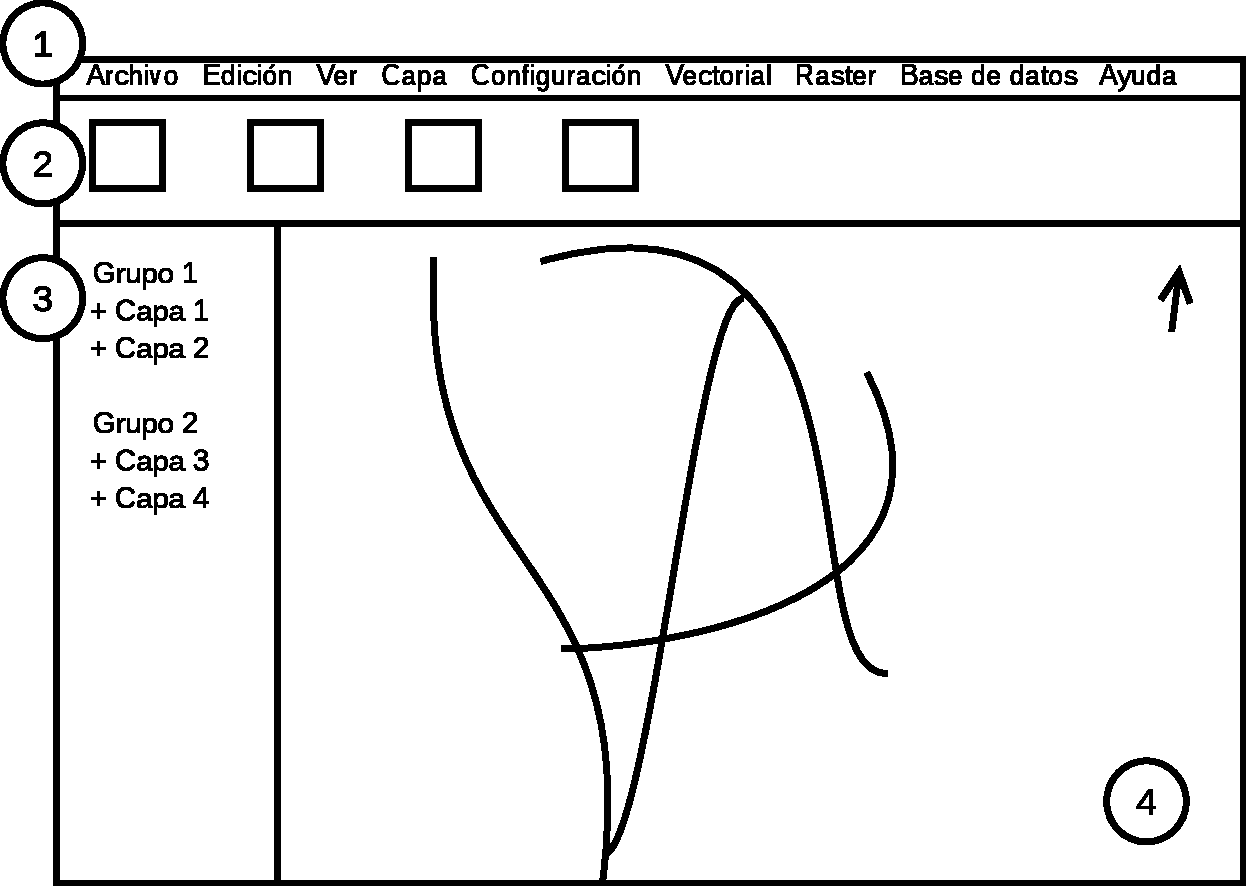
\includegraphics[scale=0.4]{gis_app}
\end{figure}

Este tipo de aplicaciones gráficas permite trabajar con capas, es decir, se pueden apilar distintos
mapas para obtener una visión completa, como podría ser el caso de un mapa que incluya la división
por predios de Valdivia superpuesto a un mapa que incluye la división por Unidades Vecinales de
Valdivia. El cruce visual de información es más simple de entender.

\subsection{Datos GIS}
Todos los datos que se trabajan en GIS son georeferenciados, es decir, contienen dentro de su
composición información relativa a su ubicación espacial. En el cuadro~\ref{datosgeo} se pueden
observar las filas de una tabla de una base de datos espacial en la que se almacenan puntos
específicos de un mapa.

\begin{table}[h]
  \centering
  \caption{Ejemplo de tabla con datos georeferenciados}
  \label{datosgeo}
  \begin{tabular}{|l|l|l|}
    \hline
    \textbf{Latitud} &  \textbf{Longitud}  & \textbf{Elemento} \\ \hline
    26.864239 & -35.898252 & Escombros \\
    34.221233 & -38.992713 & Paradero de micros \\
    26.921787 & -37.981889 & Bache \\
    \hline
  \end{tabular}
\end{table}

Los datos georeferenciados corresponden a la \emph{Latitud} y \emph{Longitud}. GIS permite mezclar
estos datos georeferenciados con otro tipo de información, como es el caso de la columna
\emph{Elemento}. Sin embargo, la potencialidad de GIS se descubre al hacer el cruce de información
entre elementos de bases de datos espaciales con otro tipo de bases de datos, como puede ser una
base de datos relacional que almacena información específica.

Los datos en GIS son almacenados en bases de datos espaciales, que tienen una estructura similar a
la mostrada en el cuadro~\ref{datosgeo}, esta base de datos espacial se puede definir de dos
maneras: (1) vectorial o (2) raster.

Los datos vectoriales son almacenados en pares de coordenadas X e Y dentro de la memoria del
computador. Los vectores son utilizados para representar puntos, líneas, polilíneas y áreas. Este
es el tipo de datos más utilizado y más flexible para su estudio y análisis. En la figura~\ref{mapa}
se pueden ver estos elementos marcados en un mapa vectorial.

\begin{figure}[h]
  \centering
  \caption{Ejemplo de mapa vectorial con áreas, polilíneas y puntos}
  \label{mapa}
  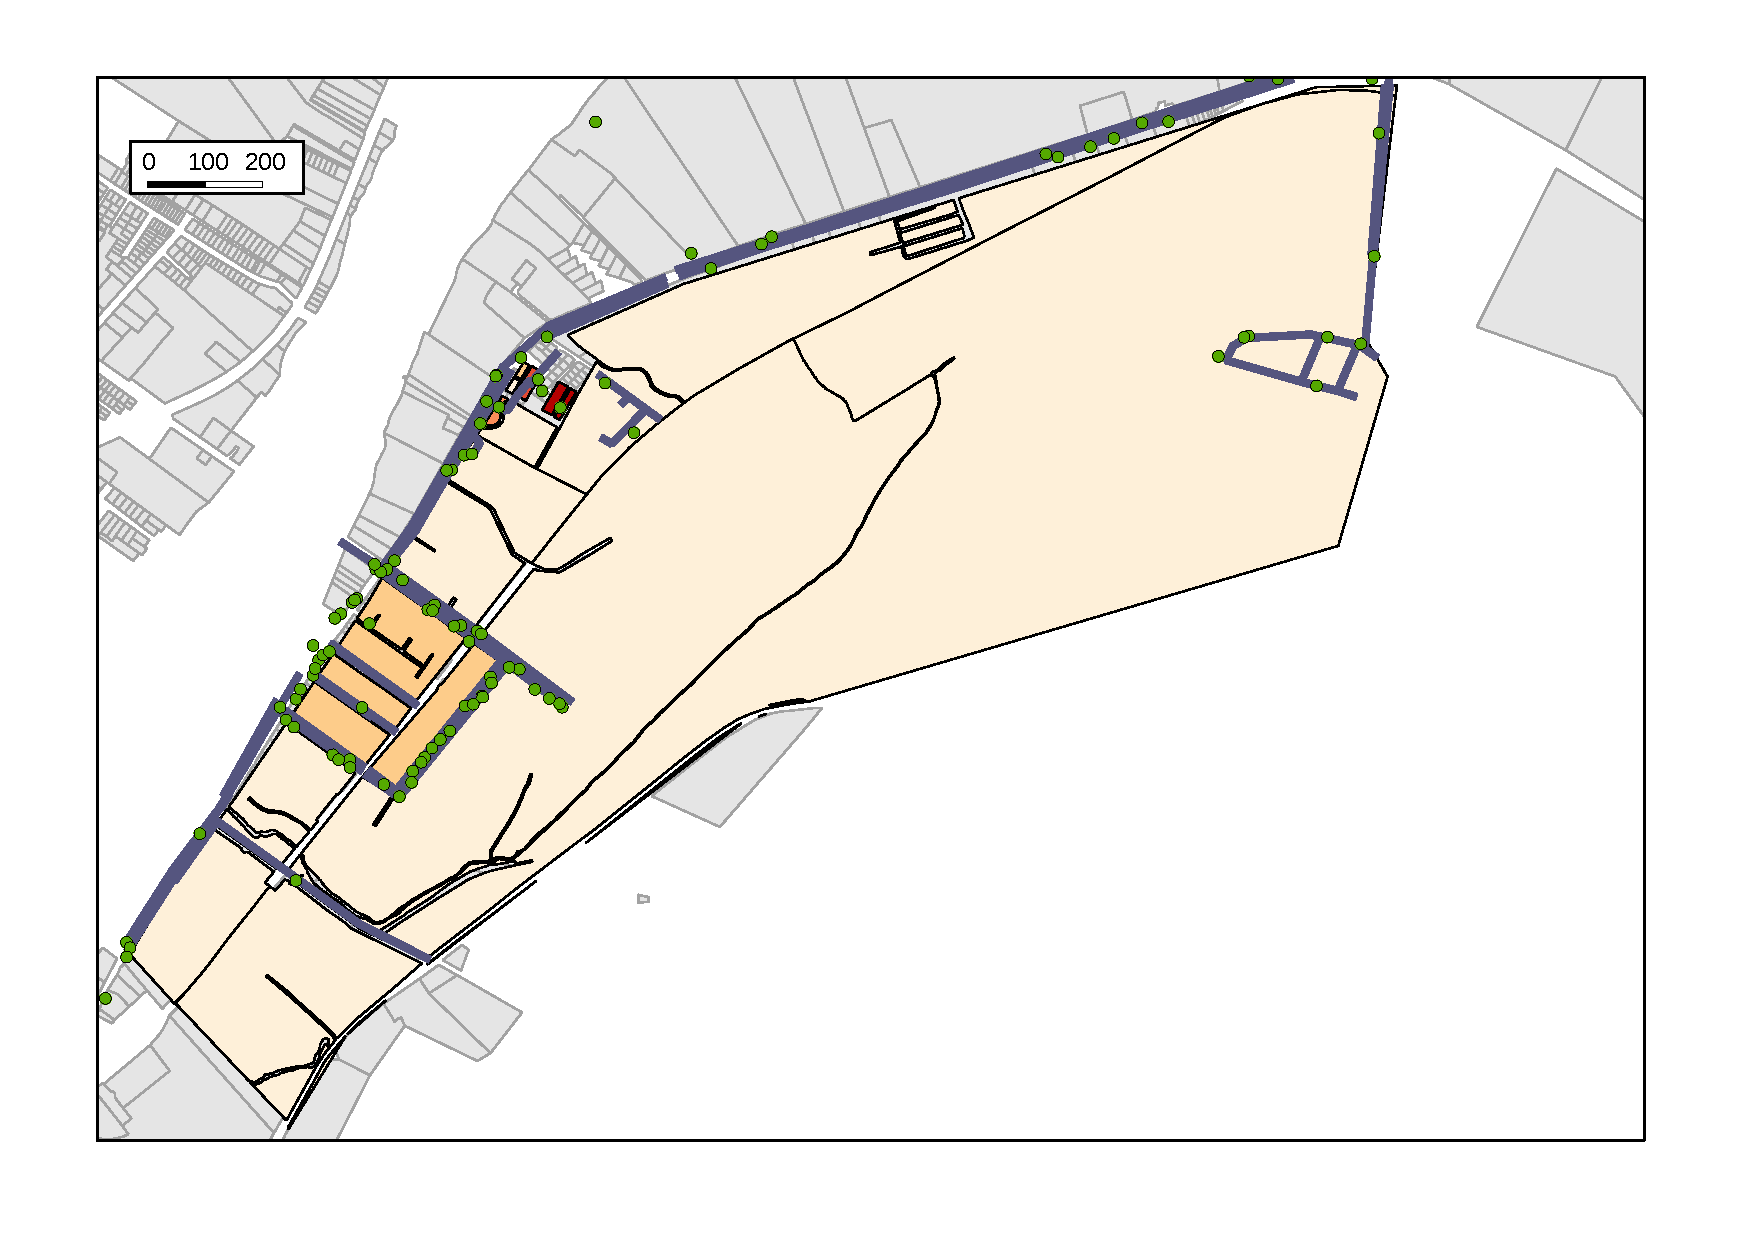
\includegraphics[scale=0.4]{mapa}
\end{figure}

Los datos de tipo raster son solo imágenes que incluyen un vector de referencia geográfica para
poder ubicarlo en las coordenadas del mapa. No son muy flexibles, pero sirven, por ejemplo, para
posicionar una capa con la imagen satelital de Valdivia y sobre ella ir trabajando con capas
vectoriales.

\subsection{Datos Vectoriales}

Los datos vectoriales permiten abstraer elementos del mundo real en una plataforma GIS, estos
elementos poseen atributos y son representados usando una geometría. Esta geometría es echa
interconectando uno o más vértices. Un vértice describe una posición en el espacio usando
coordenadas X, Y o, tal vez, Z. Las geometrías que incluyen un punto del eje Z son llamadas 2.5D, ya
que pueden describir la altura o la profundidad del vértice, pero no ambos.

Cuando un elemento geométrico está formado solo por un vértice, se denomina punto. Cuando consiste
en dos o más vértices se denomina polilínea. Cuando tiene cuatro o más vértices y el último vértice
es igual al primero, entonces se denomina polígono cerrado.

Cada uno de estos elementos incluye información adicional por sobre su geolocalización, a este tipo
de elementos se le llama base de datos espacial.

\subsection{Almacenamiento de Datos}
Existen dos mecanismos ampliamente utilizados para almacenar la información de los Sistemas de
Información Geográfico, cada uno con sus particularidades. La primera forma es a través de archivos,
como si se guardase un documento en algún software de procesamiento de palabras, por lo general se
utiliza el formato \emph{shape} de ESRI. Este formato
incluye tres tipos de archivos que corresponden a:
\begin{description}
  \item[Archivo ``.dbf'':] Archivo con los atributos de los elementos en la base de datos espacial
  \item[Archivo ``.shx''] Este archivo es un índice que ayuda a la aplicación GIS a encontrar
  elementos de manera más rápida.
  \item[Archivo ``.shp''] Archivo con la geometría de los elementos en la base de datos espacial.
\end{description}

Cuando se utiliza este mecanismo para guardar los datos se dispone de una manera rápida, fácil de
usar y descentralizada. Se deben entregar los tres archivos para que se pueda acceder a los datos.

La otra manera de almacenar los datos GIS es a través de bases de datos relacionales con extensiones
a bases de datos espaciales, tal es el caso de PostgreSQL con su extensión PostGIS, que permite a
este DBMS entender el tipo de datos geométrico donde se almacena la información de
georeferenciación. La ventaja de este método es que es increíblemente versátil para cruzar
información entre distintas tablas, que no todas tienen que ser espaciales, y permite crear nuevas
capas a partir de el cruce de datos, además, la centralización de la información hace que ésta se
mantenga estable, no fragmentada. Sin embargo, requiere de una conexión a la base de datos,
requiere de conocimientos básicos de SQL para poder hacer el cruce de datos.

\begin{thebibliography}{20}

  \bibitem[Bae99]{Bae99} Baeninger, R. (1998), `Reestruturai\c{c}a\~{a} Urbana: algumas  considera\c{c}\~{o}es  sobre o   debate actual. NEPO/UNICAMP, (mimeo) ''
  \bibitem[Car96] {Car96} Carlos, A.F. (1996), \emph{``A natureza do espac\c{c}o fragmentado''}, en:  Santos, M., Souza, M.A.A. e Silveira, M.L. (org.) \emph{Territorio: Globaliza\c{c}\~{a}o e  Fraagmenta\c{c}\~{a}o}. Editorial Hicitec-Anput, S\~{a}o Paulo 1996 (2da Edi\c{c}\~{a}o)
  \bibitem[Cas89]{Cas89} Castells, M. (1989), The Informational City, Information Technology,   economic restructuring and the urban-regional process Oxford, Basil,  Blackwell. 
  \bibitem[Cas99]{Cas99} Castells M. (1999), ``A Sociedade, Rede.Editora Paz e Terra, S\~{a}o  Paulo.'' 
  \bibitem[Ded99]{Ded99} Dedecca,C.S. y Baltar, P.E.A.(1999), ``Mercado de Trabalho e  Informalidade nos anos 90, IE/UNICAMP   (mimeo).''
  \bibitem[Gwy99]{Gwy99} Gwynne, R.N.(1999), ``Globalization, Neoliberalism and Economic Changes in  South America and  Mexico''
  \bibitem[Lat94]{Lattes}Lattes, A. E. y Z. Recchini de Lattes, Z. Recchini de Lattes
   International migration in Latin America: patterns, determinants and policies. En Naciones   Unidas, International migration: regional processes and responses, Economic Studies No. 7.   Ginebra, Comisión Económica de las Naciones Unidas para   Europa y Fondo de Población de las Naciones Unidas.
  \bibitem[Mil00]{Mil00} Mills, E.S.(2000), ``The importance of large urban areas and governments:  roles in fostering them, In: Yusuf,   S., Wu, W. and Evenett (ed.) Local Dynamics in an Era of Globalization: 21st Century Catalysts for   Development, Oxford University Press, New York. 
  \bibitem[Pav96]{Pav96} ``A lógica da periferiza\c{c}\~{a}o em áreas metropolitanas'', en Santos,  M., Souza, M.A.A. e Silveira M.L. (org.) \emph{Territorio: Globaliza\c{c}\~{a}o e  Fragmenta\c{c}\~{a}o}. Editora Hicitec-Anpur, S\~{a}o Paulo 1996 (2da Edi\c{c}\~{a}o)
  \bibitem[Rod97]{Rod97} Rodríguez J. y Villa M. (1997) ``Distribución espacial de la población,  urbanización y ciudades intermedias: hechos en su contexto''
  \bibitem[Wkur]{Wkus}{Wikipedia: Urbanismo\\ Disponible en http://es.wikipedia.org/wiki/Urbanismo}
  \bibitem[Wkuv]{Wkuv}{Wikipedia: Urbanización\\ Disponible en http://es.wikipedia.org/wiki/Urbanización}
  \bibitem[Won99]{Won99} Wong-Gonzáles, P. (1999), ``Globalización y virtualización de la economía:  impactos territoriales, V  Seminario de la Red Iberoamericana de Investigadores sobre  Globalización y Territorio. Universidad  Autónoma de México; Toluca.''



\end{thebibliography}

\end{document}
